\documentclass[]{article}
\usepackage{amsmath, mathrsfs, tikz, caption, amssymb, fancyhdr, 	epstopdf, geometry, hyperref, float, siunitx}
\usepackage{graphicx}
\usepackage{caption}
\usepackage{subcaption}
\usepackage[sort,nocompress]{cite}
\usepackage{matlab-prettifier}
\usepackage{titling}

\newcommand{\subtitle}[1]{%
 	\posttitle{%
		\par\end{center}
		\begin{center}\large#1\end{center}
		\vskip0.5em}%
}

\hypersetup{
	colorlinks = true,
	linkcolor = {blue},
	linkbordercolor = {white}
}

\geometry{a4paper, portrait, margin=1in}

\numberwithin{equation}{subsection}
\numberwithin{figure}{subsection}
\captionsetup{labelfont=bf}
\graphicspath{ {figures/} }

\usepackage{listings}
\lstset{
    	language=Matlab,                		% choose the language of the code
    %	basicstyle=10pt,       				% the size of the fonts that are used for the code
    	numbers=left,                  			% where to put the line-numbers
    	numberstyle=\footnotesize,      		% the size of the fonts that are used for the line-numbers
    	stepnumber=1,                   			% the step between two line-numbers. If it's 1 each line will be numbered
    	numbersep=5pt,                  		% how far the line-numbers are from the code
    %	backgroundcolor=\color{white},  	% choose the background color. You must add \usepackage{color}
    	showspaces=false,               		% show spaces adding particular underscores
    	showstringspaces=false,         		% underline spaces within strings
    	showtabs=false,                 			% show tabs within strings adding particular underscores
    %	frame=single,	                			% adds a frame around the code
    %	tabsize=2,                				% sets default tabsize to 2 spaces
    %	captionpos=b,                   			% sets the caption-position to bottom
    	breaklines=true,                			% sets automatic line breaking
    	breakatwhitespace=false,        		% sets if automatic breaks should only happen at whitespace
    	escapeinside={\%*}{*)}          		% if you want to add a comment within your code
    }

\renewcommand{\thesubsection}{\thesection.\alph{subsection}}
\newcommand{\lapL}[1]{\mathscr{L}\{#1\}}
\setlength{\parindent}{0pt}

\pagestyle{fancy}
\fancyhf{}
\setlength{\headheight}{25pt}
\lhead{MTRX5700 Major Project}
\rhead{Neill Foweraker 430225437\\Angus Mitchell 440246554\\Xue Yin Zhang 440305585}
\rfoot{Page \thepage}

%opening
\title{Do a Flip}

\subtitle{MTRX5700 Experimental Robotics\\Major Project}
\author{Neill Foweraker 430225437\\Angus Mitchell 440246554\\Xue Yin Zhang 440305585}

\begin{document}

\maketitle

\tableofcontents
\listoffigures
\newpage


\section{Introduction}
\newpage
\section{Background}
\newpage
\section{Experimental Design} % section could also be called experimental set-up
\newpage
\section{Results}

% \subsection{Program Design}

%%NOT SURE IF THIS IS NECESSARY IN RESULTS

\subsection{Sound Processing}

%%ANGUS: for you to discuss how we achieved what's been specified in the intro - make subsubsections for like brief description of how we're using aubio, beat detection, clustering, etc...

%% fix the intro/background if you feel inaccurately describes the sound processing bits (doesn't need to be too detailed in the intro/background) - your time to shine is here and in section 4

Some sound processing modules were implemented sucessfully, while others were not perfect, requiring further refinement. The module that worked very effectivly was beat detection. Switching from tempo to onset detection worked very effectivly for song sections that did not contain a distinct beat, or sections with a changing tempo. Clustering of song sections also worked effectivly, providing a nice way to divide the song up into distinct and useable sections (see figure \ref{fig:cluster_output} and \ref{fig:clustering}). The component that was less affective was the classification. In hindsight, changed could have been made in the classification module to achieve more accurate and useful results. \\
\\
\begin{figure}[H]
      \centering
      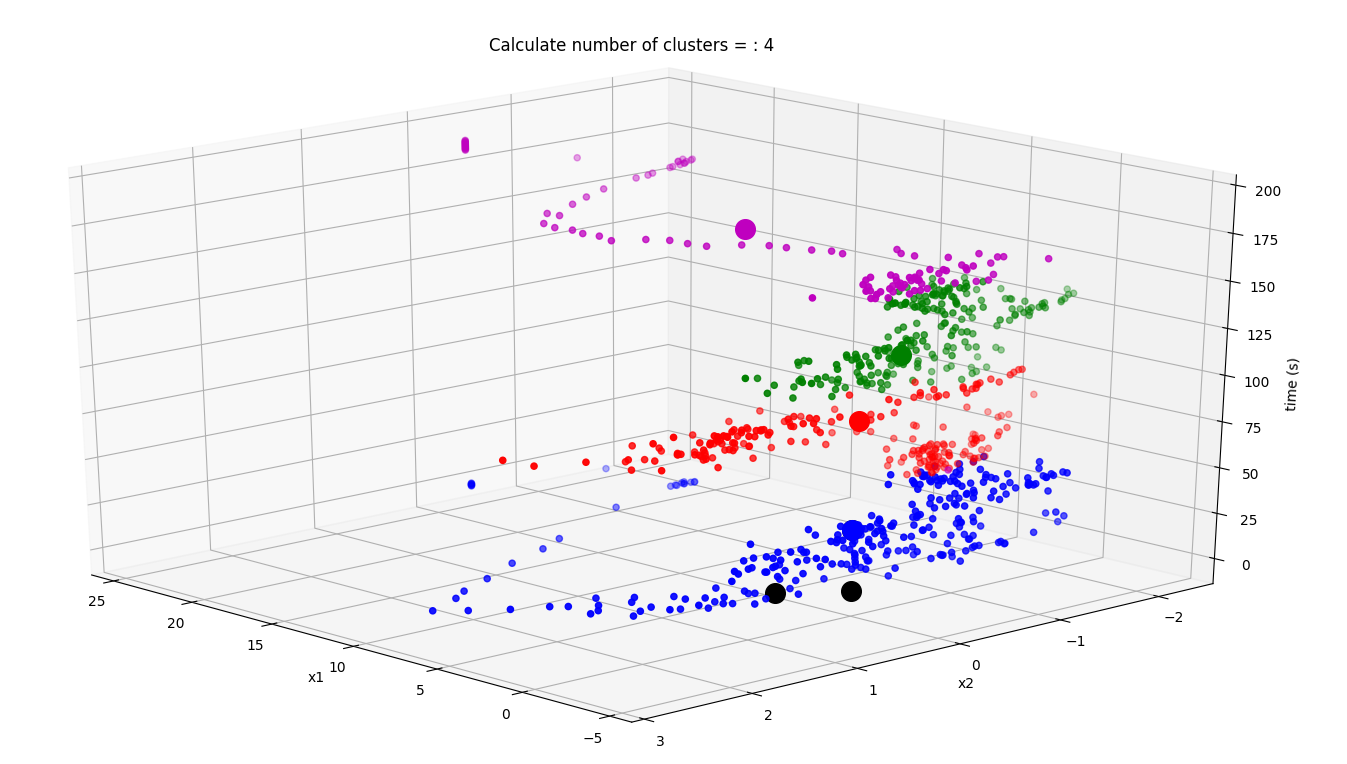
\includegraphics[width=1\linewidth]{clustering.png}
      \caption{Clustering results: the song is divdied into distinct sections. Each colour represents a different cluster, with the cluster centroid represented by the larger markers. x1 and x2 axes represent the reduce feature set, while the vertical axis is time.}
      \label{fig:clustering}
\end{figure}
\begin{figure}[H]
      \centering
      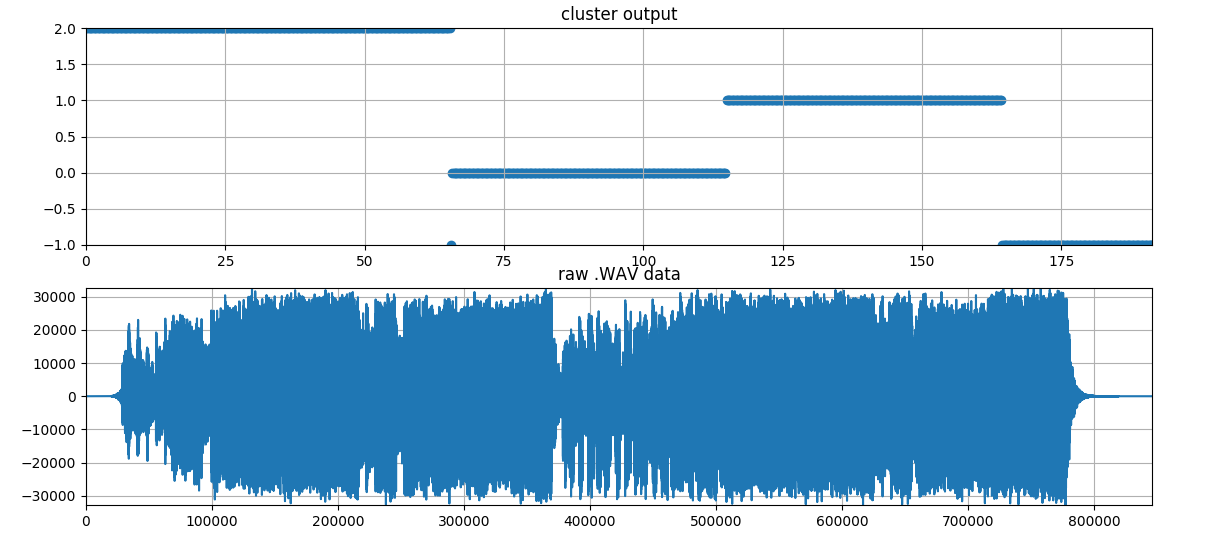
\includegraphics[width=1\linewidth]{cluster_output.png}
      \caption{An alternate view of the clustering results. The cluster number is plotted next to the raw song data.}
      \label{fig:cluster_output}
\end{figure}



\subsection{Latency Management}

% we can talk about system performance by pulling some numbers out of our ass (like numbers in the same ballpark as we were getting when timing how long it took for a packet to send)

% and other things

\onecolumn

\begin{multicols}{2}
\subsection{Space Confinement}

For this module, we successfully configured the drone to receive and decode the navigation data packages that were being sent from the drone to the laptop. The three datasets which were useful to this module are shown in Figure \ref{fig:4c-sample-nav}.

\begin{figure}[H]
      \centering
      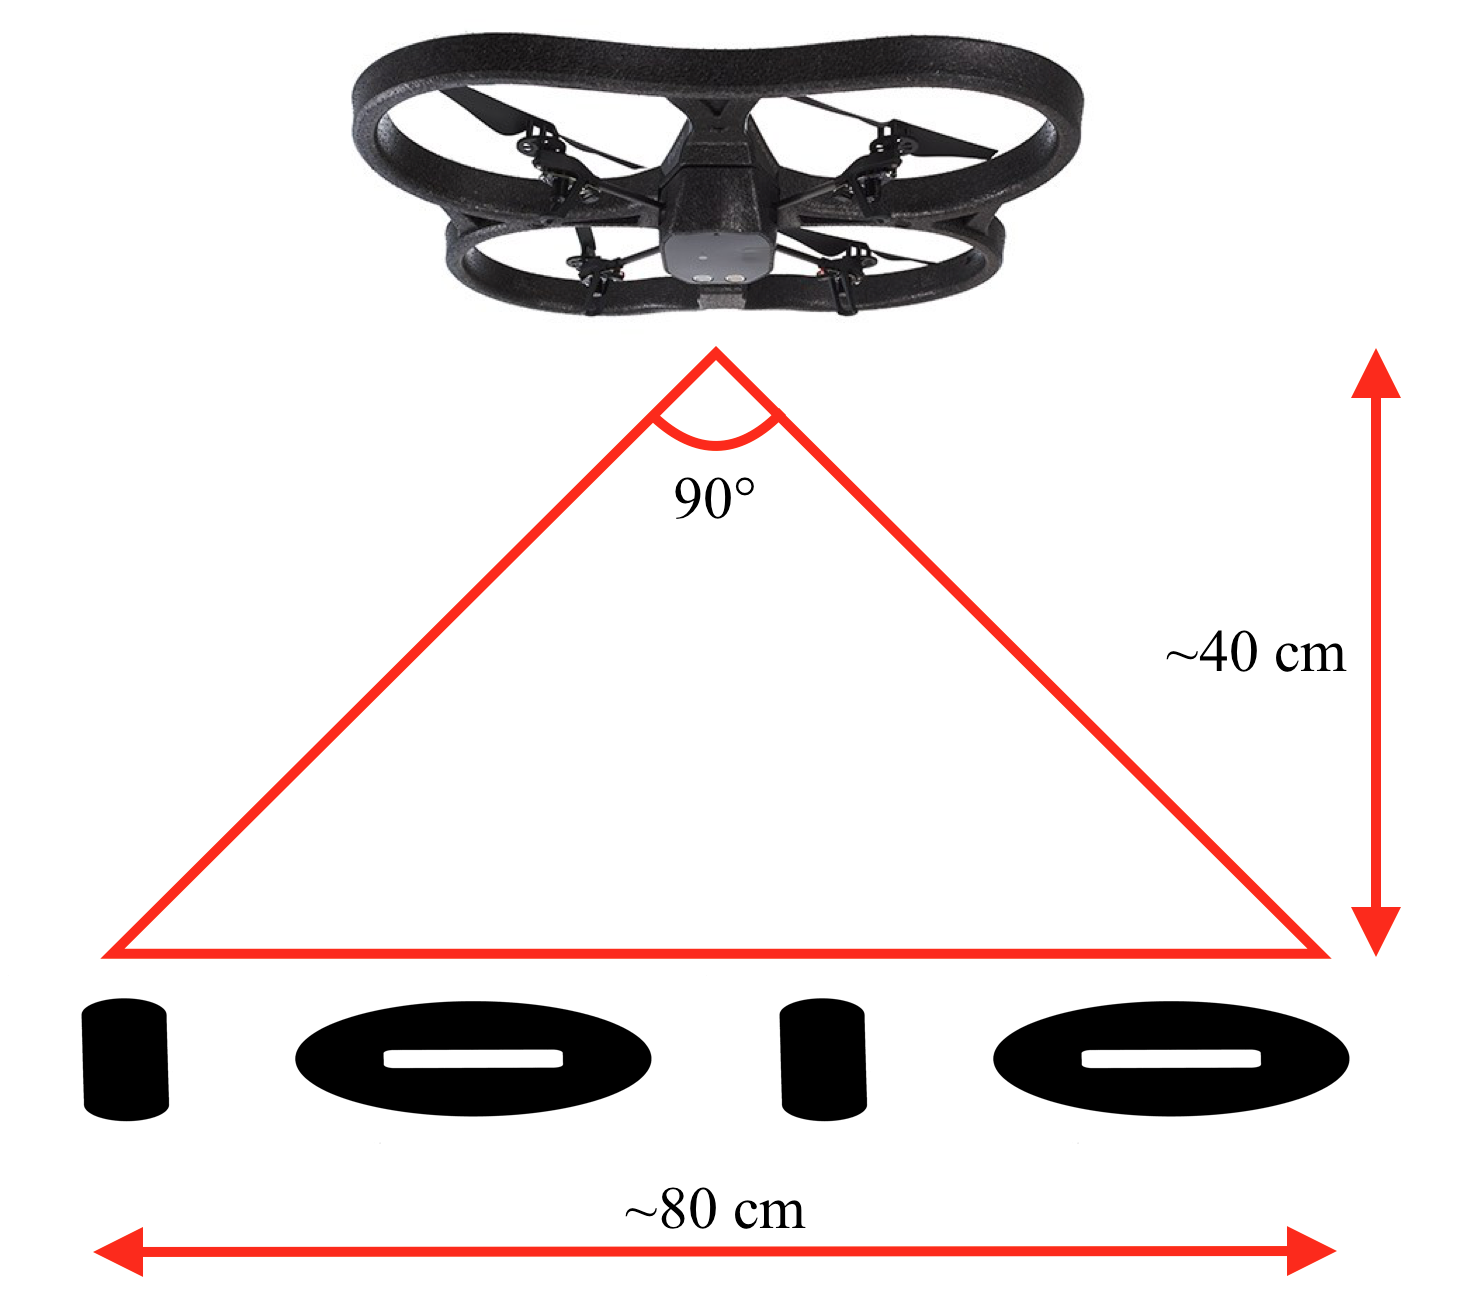
\includegraphics[width=0.8\linewidth]{3d-drone-fov.png}
      \caption{Sample navigation data from the drone when rotating clockwise near a roundel}
      \label{fig:4c-sample-nav}
\end{figure}

The following figure includes a few screenshots from a video where the drone approaches a row of roundels, and then backs away again.

\end{multicols}
\begin{figure}
        \begin{subfigure}[b]{0.25\textwidth}
                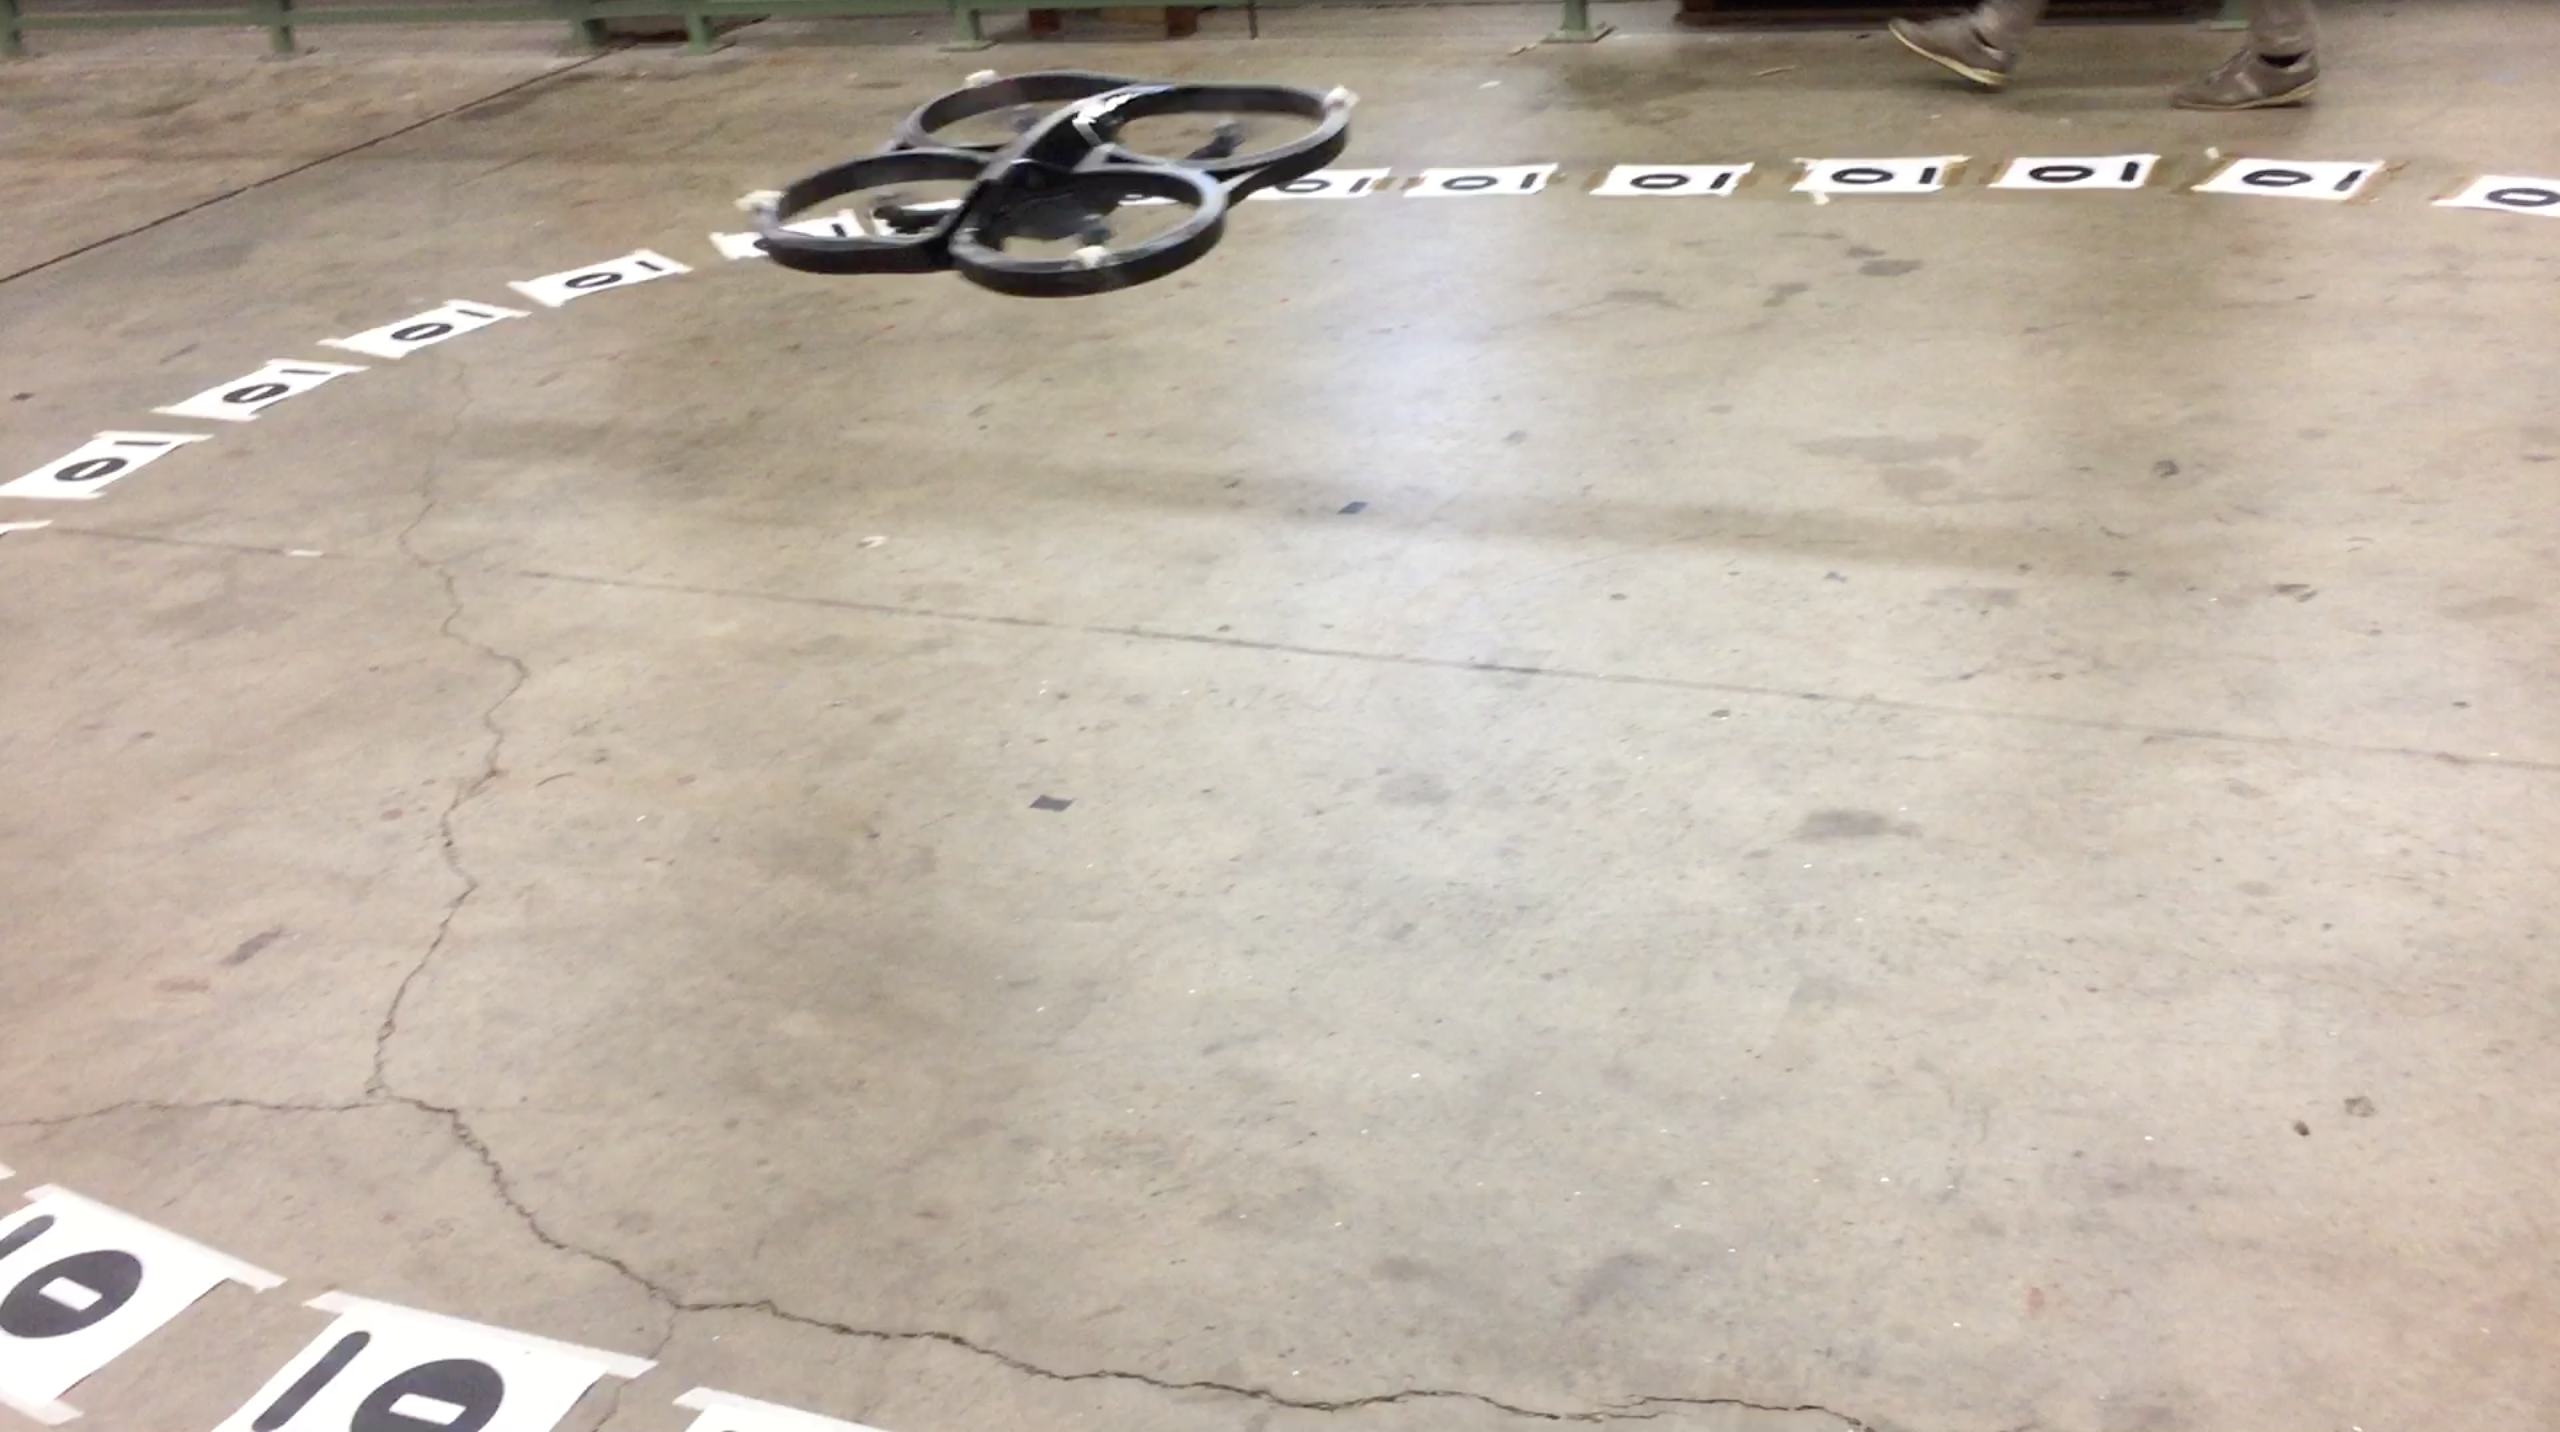
\includegraphics[width=\linewidth]{4c-flying-towards.png}
                \caption{Drone is flying towards the roundel boundary}
        \end{subfigure}%
        \hspace{\fill}
        \begin{subfigure}[b]{0.25\textwidth}
                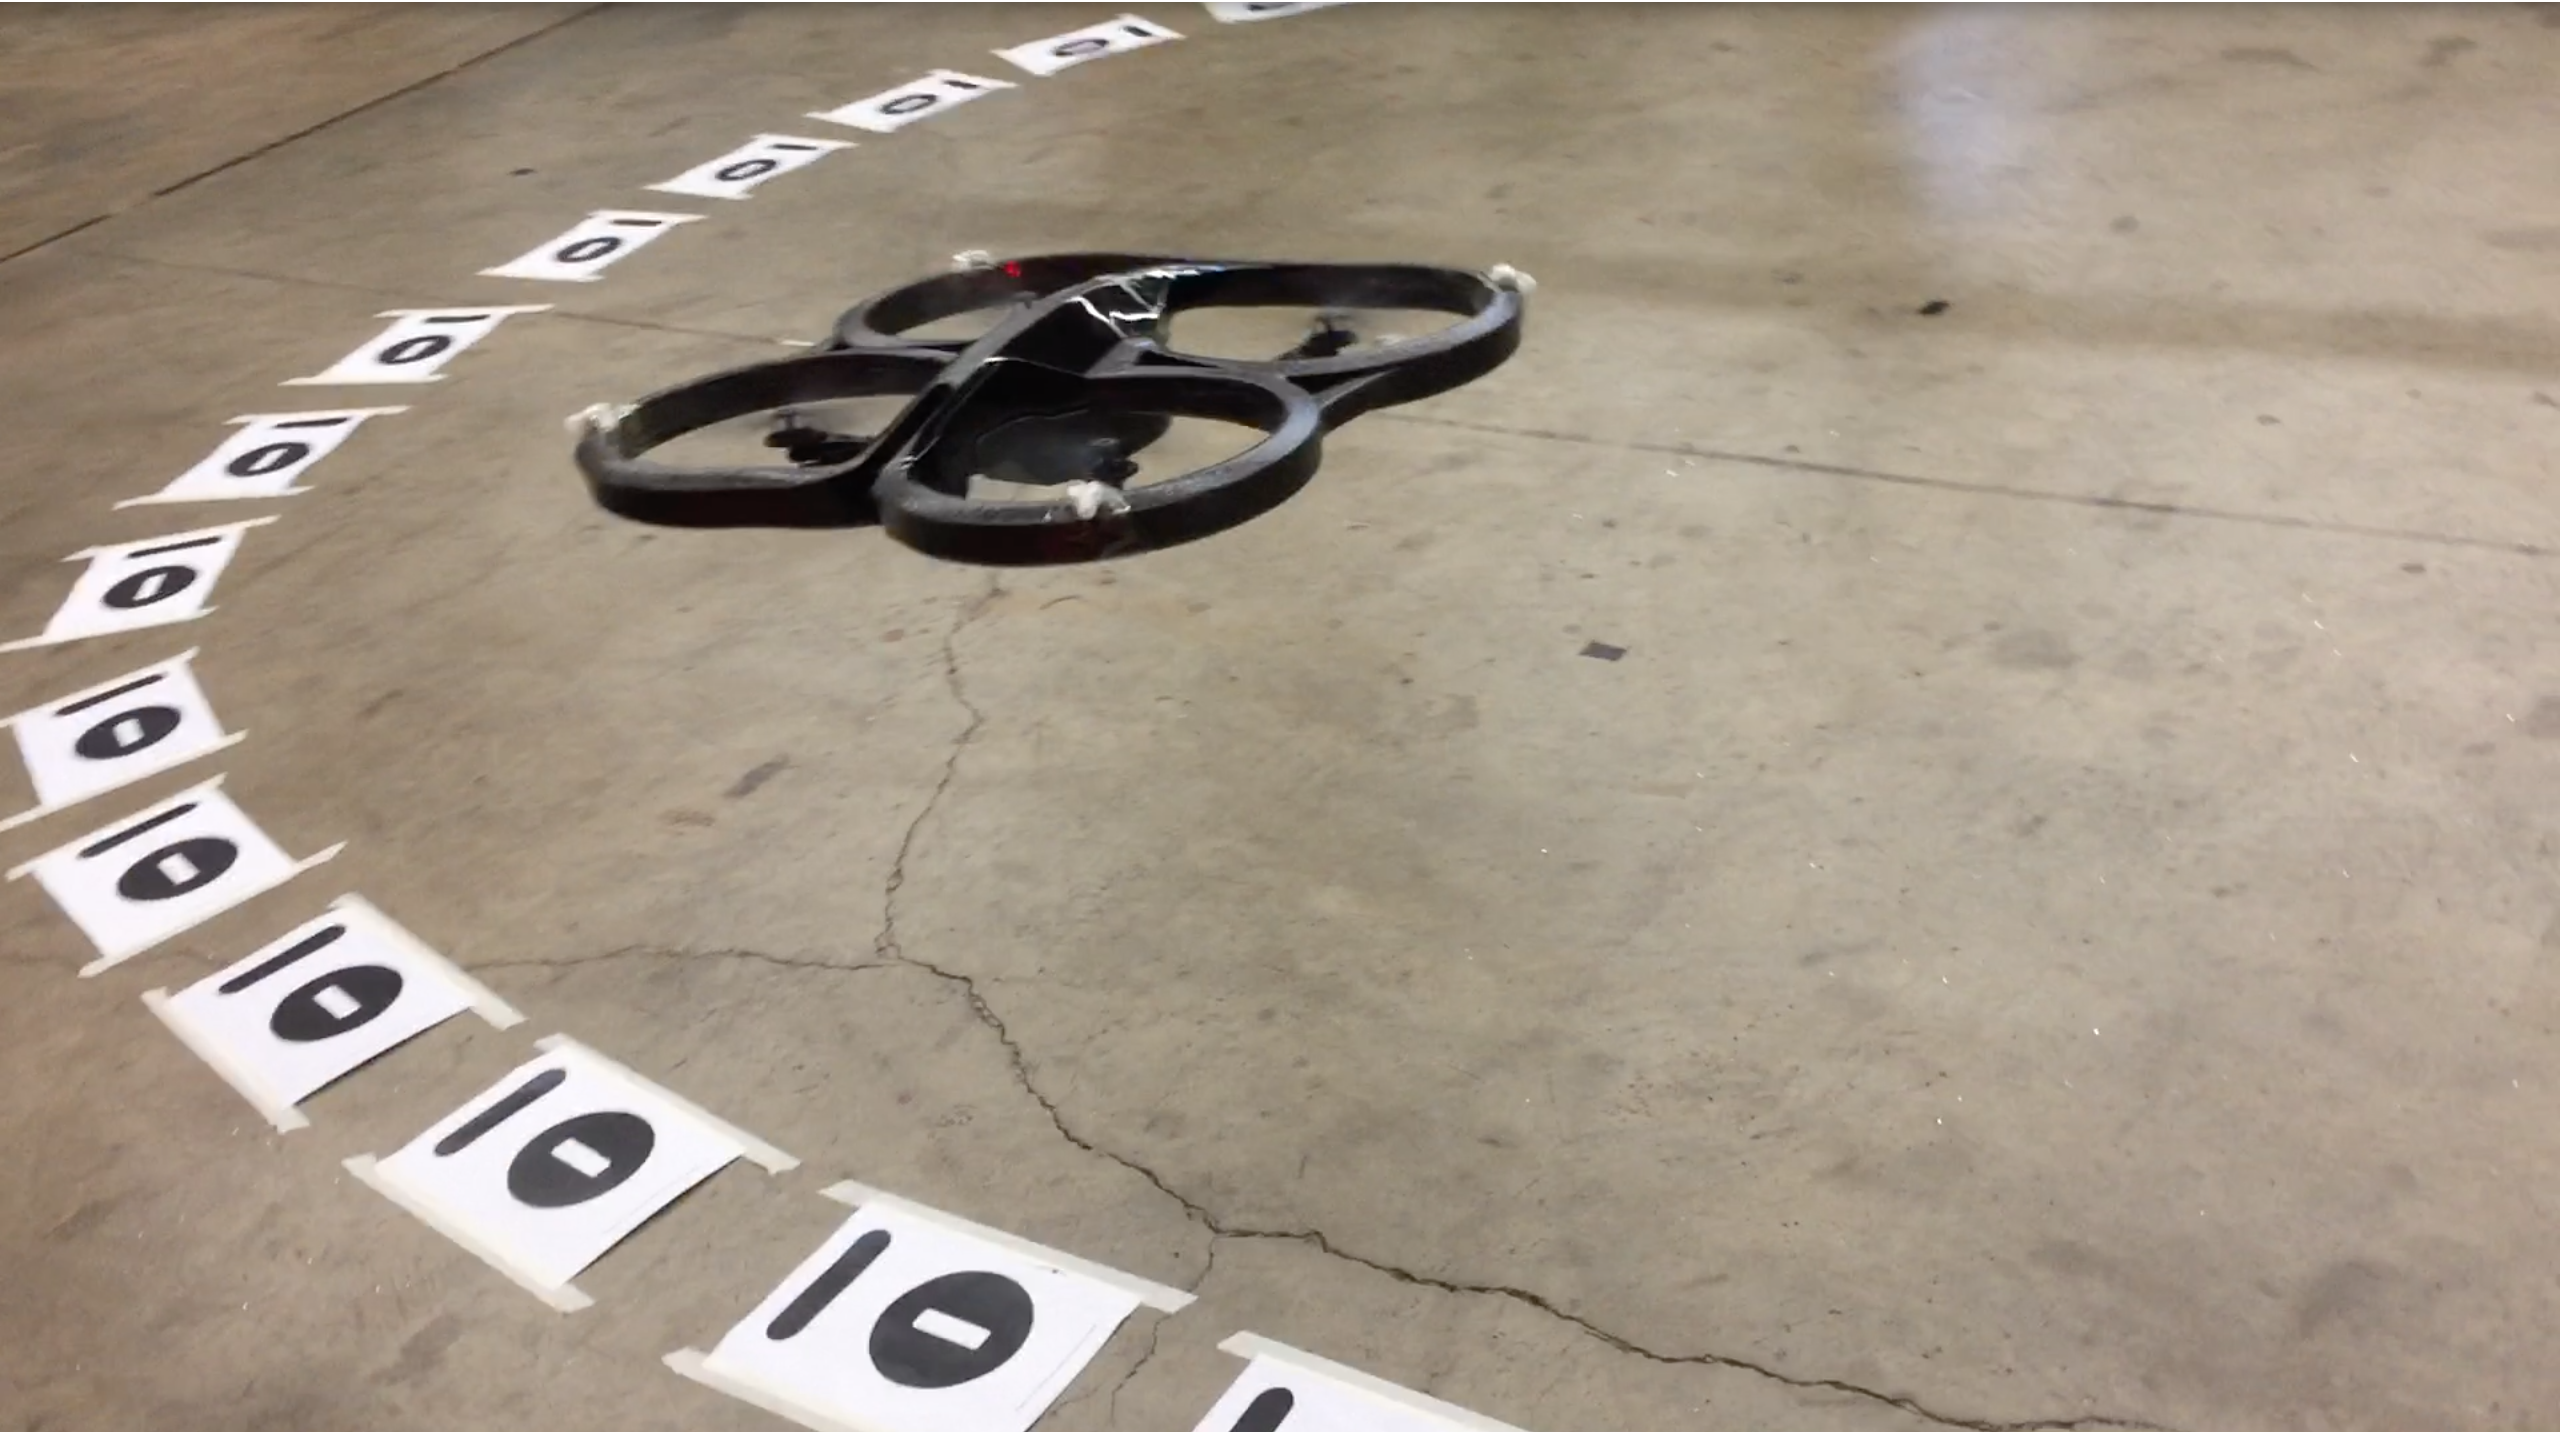
\includegraphics[width=\linewidth]{4c-found-boundary.png}
                \caption{Drone has detected a roundel at the boundary}
        \end{subfigure}%
        \hspace{\fill}
        \begin{subfigure}[b]{0.25\textwidth}
                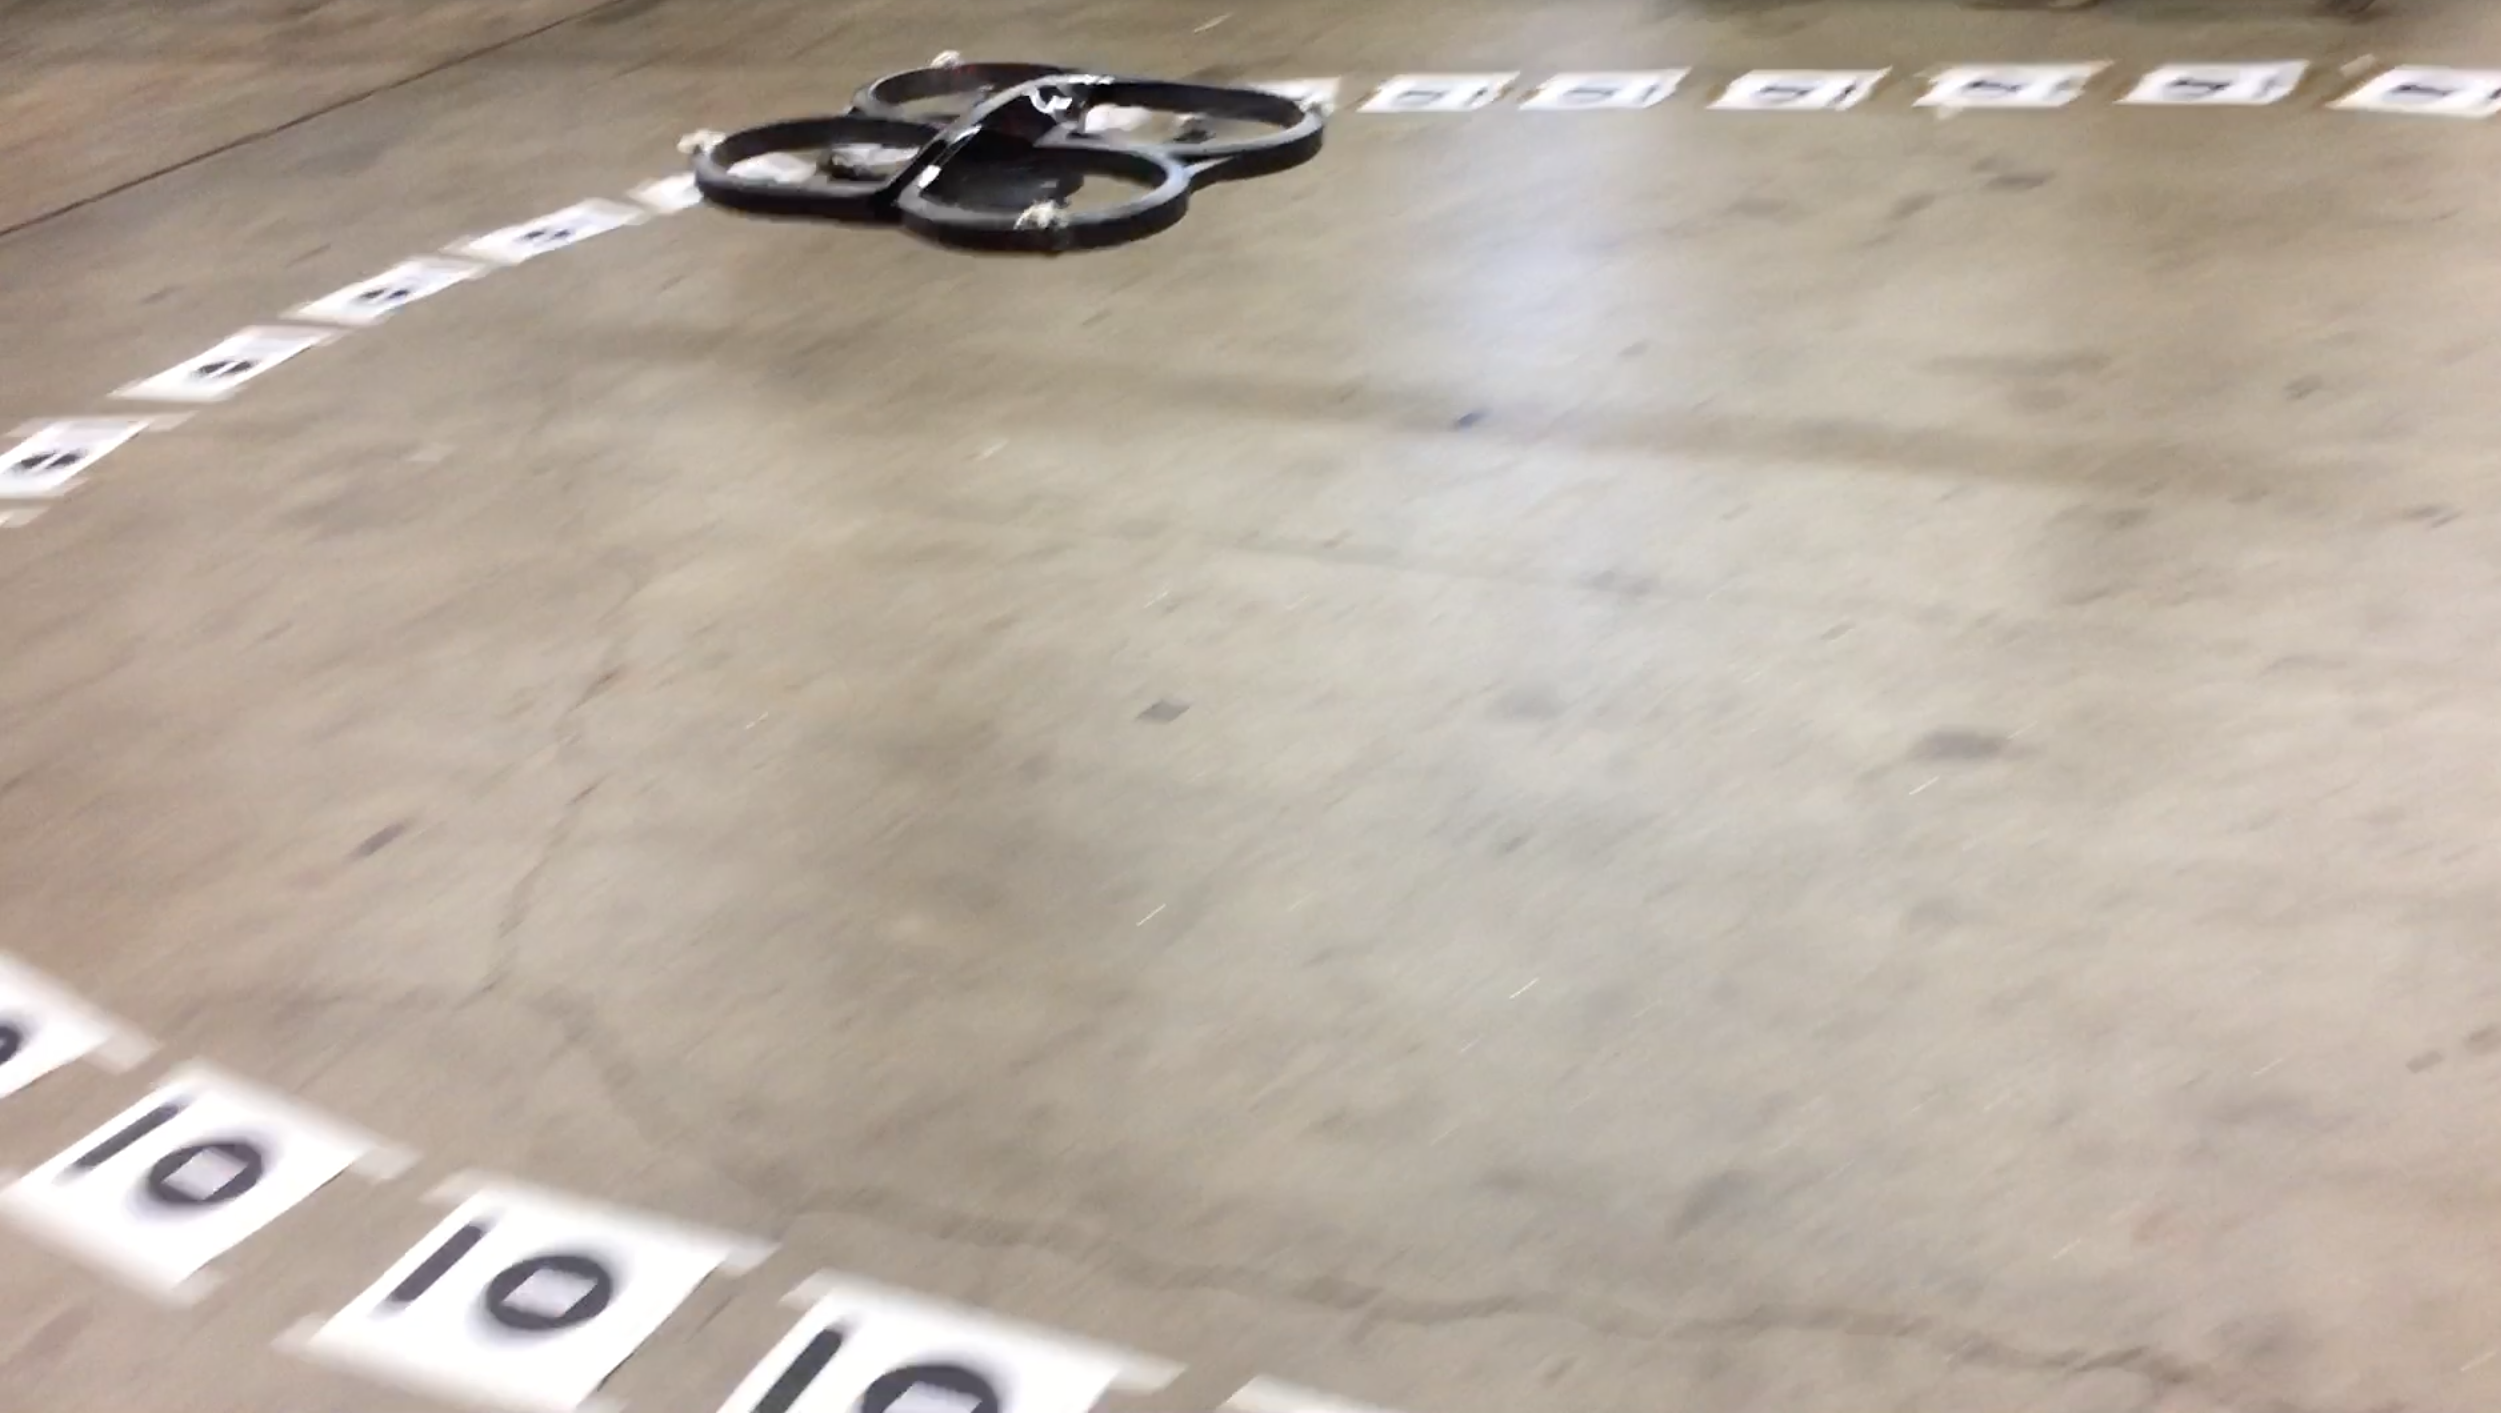
\includegraphics[width=\linewidth]{4c-backing-away.png}
                \caption{Drone is now backing away from the roundel}
        \end{subfigure}
        \caption{Screenshots from a video}\label{fig:4c-video}
\end{figure}
\twocolumn

\newpage
\section{Discussion}
\newpage
\section{Conclusions} % section could also be called future work

%\subsection{Future Work}

\bibliographystyle{plain}
\bibliography{biblio}

\end{document}
